\section{Linear System of ODEs}

A differential equation of the form
$$ X' = A(t) X + f(t) $$
where $A(t)$ is an $n \times n$ matrix and $f$ is a map from an interval $I \subset \R$ to $\R^n$ is known as a linear system of ODEs. $A(t)$ is called the matrix of coefficients (its entires being the coefficients) and the function $f$ is called the inhomogeneity. If $f = 0$ then the equation is called homogeneous and if $A(t)$ is a constant matrix then we have what is called a constant coefficient ODE. As usual, if $X' = F(X)$ for some $F$, then all $X_0$ that satisfy $F(X_0) = 0$ are called equilibrium points of a system (in the case of a linear system, $F(X) = A(t) X + f(t)$, but this statement applies more generally). 

We will start by considering the simplest case of a linear system: a homogeneous, constant coefficient ODE (as we will see solving a homogeneous ODE allows us to solve the general system, see \autoref{sec:superposition-principle}). In this case $X_0 = 0$ is always a equilibrium point. If $\det(A) = 0$ then we have a space of equilibrium. Reducing further to case of $A$ being $2 \times 2$, if $\det(A) = 0$ we have a straight line of equilibrium points in $\R^2$ (we of course ignore the uninteresting case of $A = 0$).\\

As mentioned, we will start by simply considering the case in $\R^2$. In other words our differential equation is of the form
\begin{equation}\label{eq:hom-lin-eqn}
    \matrix{x \\ y}' = \underbrace{\matrix{a & b\\c & d}}_{A} \matrix{x \\ y} = \matrix{ax + by \\ cx + dy}
\end{equation}
The system would be easy to solve if $b = 0$ and $c = 0$ as we would left with equations of the form $x' = ax$ and $y' = dy$ which already know how to solve. This occurs if $A$ is a diagonal matrix. If $A$ is diagonalizable, then we can change our coordinates to make $A$ diagonal and solve the system. In either case, we more or less get $x = x_0 e^{at}$ and $y = y_0 e^{dt}$ as our general solutions. Moreover, in the one-dimensional, case the system would would look like $x' = ax$, which again has the solution $x(t) = x_0 e^{at}$. This might inspire us to define the answer for the $2 \times 2$ case (and the general case) to be
$$ X(t) = e^{At} $$
Despite the nonsense that this looks, there is a way of interpreting what it means to ``exponentiate a matrix", using the Taylor expansion of $e^x$. In other words, we define
$$ e^{At} := \sum_{k = 0}^{\infty} \frac{t^k}{k!} A^k = I + tA + \frac{t^2}{2}A^2 + \frac{t^3}{3!} A^3 + \dots $$
Of course this is an infinite series so we need to decided whether it converges or not (and what convergence even means in this case), but at least each of the terms in the series makes sense.

As we will see later, this is in fact always convergent and does indeed solve our ODE and forms a general solution to our ODE. Moreover, we have that
$$ \frac{d}{dt} e^{At} = A e^{At} $$

Another educated guess one may make, once again looking at the one-dimensional case, is that the answer will be of the form
$$ x(t) = e^{\lambda t} v $$
where $\lambda$ is a real number and $v$ is a (constant) vector in $\R^n$, which are parameters to be determined. Assuming this to be case, we can substitute this in \autoref{eq:hom-lin-eqn} to conclude that
$$ \lambda e^{\lambda t} v = A (e^{\lambda t} v) $$
for all $t$.
This implies that $Av = \lambda v$ or in other words that $\lambda$ is an eigenvalue with eigenvector $v$.

\subsection{Example}
Let us try our hand with an example (with the second guess for now).
Suppose we are given
\begin{equation}\label{eq:lin-eqn-eg}
    \matrix{x\\y}' = \underbrace{\matrix{2 & 3\\1 & 0}}_{A} \matrix{x\\y}
\end{equation}

Using our favourite method of finding eigenvalue/eigenvector pairs, we determine that the eigenvalues of $A$ are $3$ and $-1$ with eigenvectors $\matrix{3\\1}$ and $\matrix{1\\-1}$ respectively. We then have two solutions
\begin{align*}
    X_1(t) &= e^{3t}\matrix{3\\t}\\
    X_2(t) &= e^{-t}\matrix{1\\-1}
\end{align*}

However observe that any linear combination of $X_1$ and $X_2$ is also a solution. This leads us to superposition principle (also known as the linearity principle).

\begin{figure}[h]
    \centering
    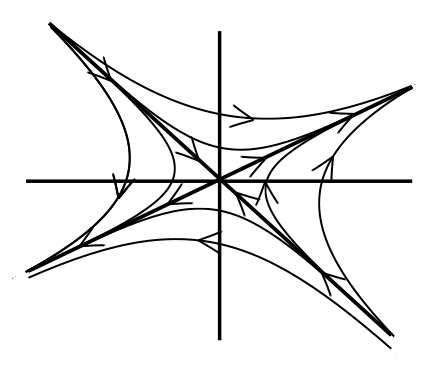
\includegraphics[scale=0.6]{Images/phase portrait.png}
    \caption{Phase Portrait of \autoref{eq:lin-eqn-eg}}
    \label{fig:phase-portrait-eg}
\end{figure}

\subsection{Superposition/Linearity Principle} \label{sec:superposition-principle}
Suppose $X_1(t)$ is such that it solves
$$ X' = A(t)X + f_1(t) $$
and $X_2(t)$ solves
$$ X' = A(t)X + f_2(t) $$
Then for real $a_1, a_2$, $X(t) = a_1 X_1(t) + a_2 X_2 (t)$ solves
$$ X' = A(t)X + a_1 f_1(t) + a_2 f_2(t) $$
This is easily verified by substituting the solution into the differential equation (and using the fact that multiplication with a matrix is linear). A consequence of this is that solutions to a homogeneous, linear system of ODEs forms a vector space. 

Another consequence is the fact that the general solution $X'(t) = A(t)X + f(t)$ is given by
$$ X(t) = X_{genhom}(t) + y(t) $$
where $X_{genhom}(t)$ is the general solution to the homogeneous system of equations $X' = AX$ and $y(t)$ is one \textit{particular} solution to $X'(t) = A(t)X + f(t)$ (recall the similarities to solving a linear system of equations given by $AX = b$, where the solution is given by $b + \tilde{X}$ where $\tilde{X}$ is the space of solutions solves $AX = 0$ (if $b$ lies in the range of $A$)).

This means that if $X$ maps to $\R^n$ and $A \in \R^{n \times n}$ then the space of solutions to $X' = AX$ forms a $n-$dimensional vector space. In fact if $X_1(t), \dots, X_n(t)$ are (linearly independent) solutions to $X' = AX$ then 
$$ X(t) = a_1 X_1(t) + \dots a_n X_n(t) \quad a_1, \dots, a_n \in \R $$
is the general solution to $X' = AX$. This in fact holds in general but we will only prove this for the case when $A$ can be diagonalised (for now). Later we will show the general case.

\begin{lemma}
The general solution to $X' = AX$ where $X$ maps to $\R^n$ and $A$ is a diagonalisable $n \times n$ matrix is given by 
$$ X(t) = a_1 X_1(t) + \dots a_n X_n(t) $$
where the $X_i$ themselves are linearly independent solutions (meaning $X_1(t), \dots, X_n(t)$ are linearly independent for all $t$) to the system of equations.
\end{lemma}
\begin{proof}
Let $v_1, \dots, v_n$ be eigenvectors of $A$ that form a basis for $\R^n$. Suppose their respective eigenvalues are $\lambda_1, \dots \lambda_n$.

Suppose the initial value problem is given by
\begin{equation}
  \left\{
  \begin{array}{@{}ll@{}}
    X' = AX \\
    X(0) = a_1 v_1 + \dots a_n v_n
  \end{array}\right.
\end{equation}
Then
$$ Y(t) = a_1 e^{\lambda_1 t}v_1 \dots a_n e^{\lambda_n t} v_n $$
solves this initial value problem.

Suppose $Z(t)$ is another solution to this IVP. Since $v_1, \dots v_n$ is a basis for $\R^n$, we can write $Z(t) = b_1(t) v_1 + \dots b_n(t) v_n$ where the $b_i$ are real-valued functions. We know that $b_i(0) = a_i$ since $Z(0) = Y(0) = X(0)$. Also note that
\begin{align*}
    Z'(t) &= b_1'(t) v_1 + \dots b_n'(t) v_n\\
    AZ(t) &= A(b_1(t) v_1) + \dots b_n(t) v_n)\\
    &= b_1 \lambda_1 v_1 + \dots + b_n \lambda_n v_n
\end{align*}
Equating coefficients of the $v_i$ (which are uniquely determined since the $v_i$ for a basis) we get that $b_i'(t) = \lambda_i b_i(t)$ and $b_i(0) = a_i$. We know that for each $i$, this is uniquely solved by $b_i(t) = e^{\lambda_i t} a_i$ implying that $Z = Y$. This allows us to conclude that the solutions to $X' = AX$ are uniquely determined by the initial value.
\end{proof}
\begin{remark}
We know that that $b_i$ above are differentiable as they are the composition of two differentiable functions: $Z$ and the linear projection onto $v_i$ which is a linear map with constant coefficients/entries (hence in particular is differentiable with respect to $t$).
\end{remark}

\subsection{Types of Systems}
We can categorise the different systems of equation based on the eigenvalues.

\subsubsection{Saddle Point}
Suppose we are given 
\begin{equation}
    X' = \underbrace{\matrix{2 & 3\\1 & 0}}_{A} X
\end{equation}
Then we know that its eigenvalues are $\lambda_1 = 3$ and $\lambda_2 = -1$ with eigenvectors $v_1 = (3, 1)$ and $v_2 = (1, -1)$ respectively. Note that this is a case where the eigenvalues are of opposite sign. In this case the phase portrait would look like \autoref{fig:saddle_point}.
\begin{figure}[h]
    \centering
    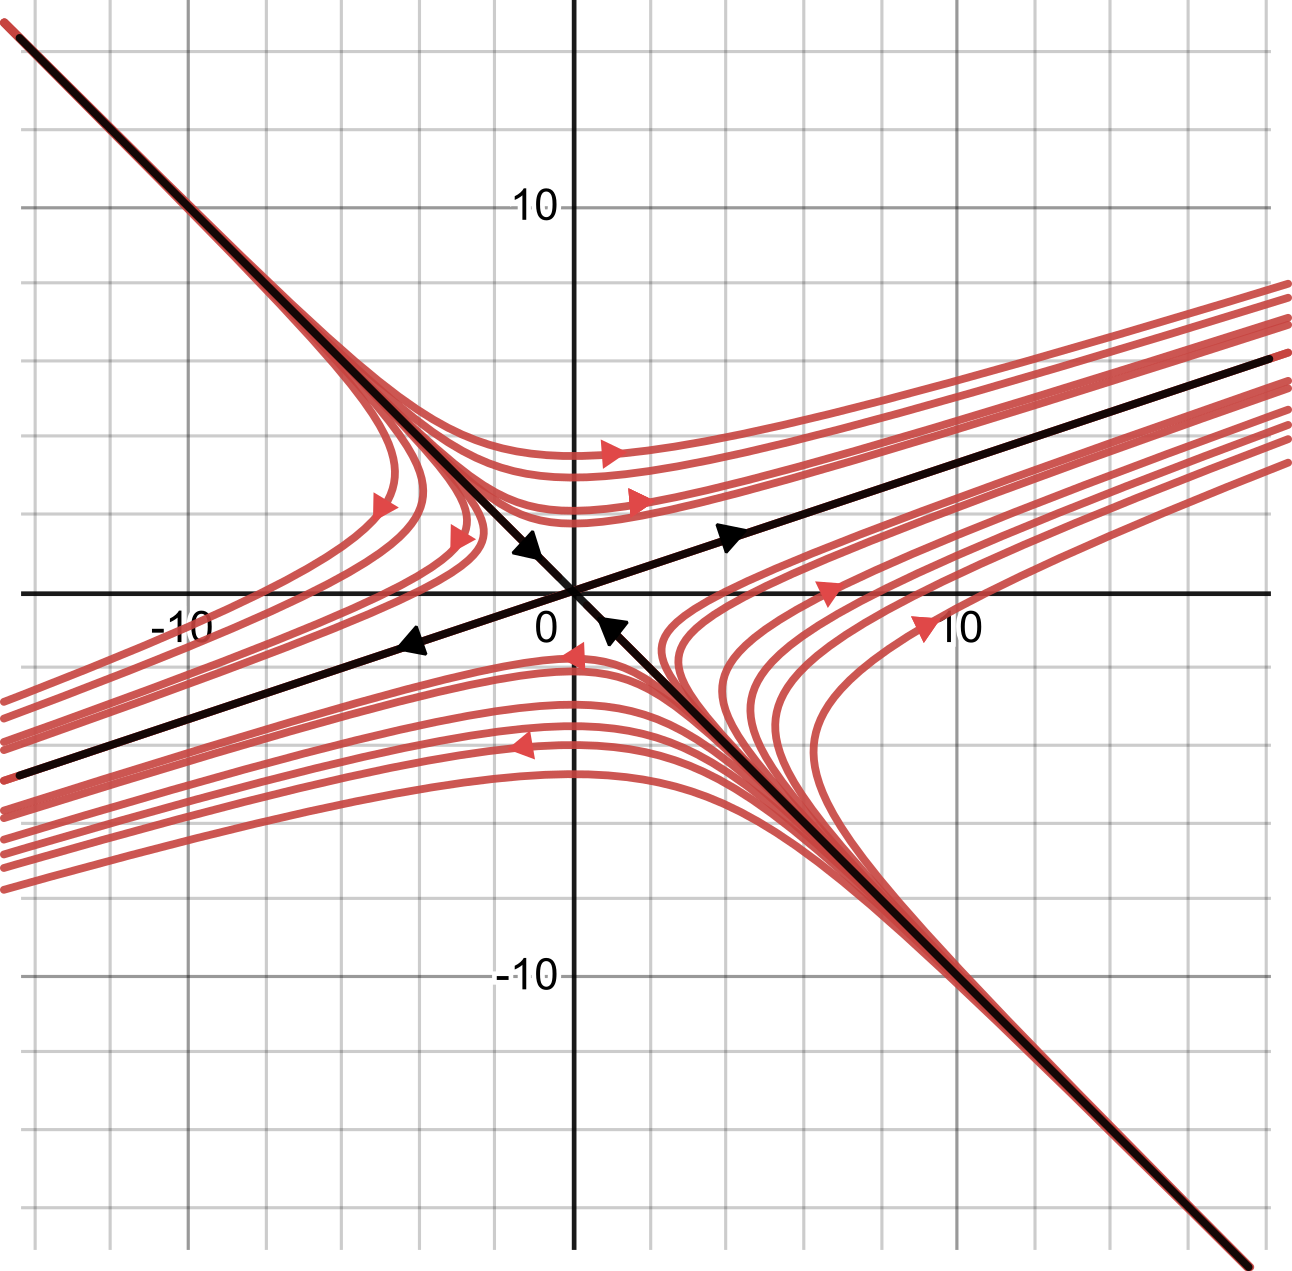
\includegraphics[scale=0.35]{Images/saddle_point.png}
    \caption{Saddle point}
    \label{fig:saddle_point}
\end{figure}

Note that as time as evolves points on the line spanned by $v_2$ move towards the origin (exponentially) while points on the line spanned by $v_1$ move away (also exponentially). In this case we call $v_2$ the stable line and $v_1$ the unstable line. Now consider a point that is not on either of these lines but is some linear combination of $v_1$ and $v_2$. In this case as time evolves, the component for $v_2$ will shrink to 0 while the component for $v_1$ will shoot off to infinity leading to this above shape. This is called having a saddle point at 0. Any time we have eigenvalues of opposite sign we get something like above.

\subsubsection{Unstable Node}
The next question, of course, is of course is what happens if we have two eigenvalues of the same sign. We first consider the case of both eigenvalues being positive. As an example, we can consider
\begin{equation}
    X' = BX
\end{equation}
where $B = A + 2I$. Then the eigenvalues of $B$ are $\lambda_1 = 5$ and $\lambda_2 = 1$ with $v_1$ and $v_2$ as before. In this case everything moves away from the origin giving us what is called an ``unstable node at 0". However note that since the $\lambda_1$ is greater, the $v_1$ component of any point will increase much faster as $t \to \infty$. So eventually the paths will seem parallel to $v_1$. Conversely as $t \to 0$, the $v_1$ component will also decrease to 0 faster than $v_2$ so the integral curves (aka solutions) become tangent to $v_2$ as $t$ approaches 0. Hence we conclude that the phase portrait will look like so.

\begin{figure}[h]
    \centering
    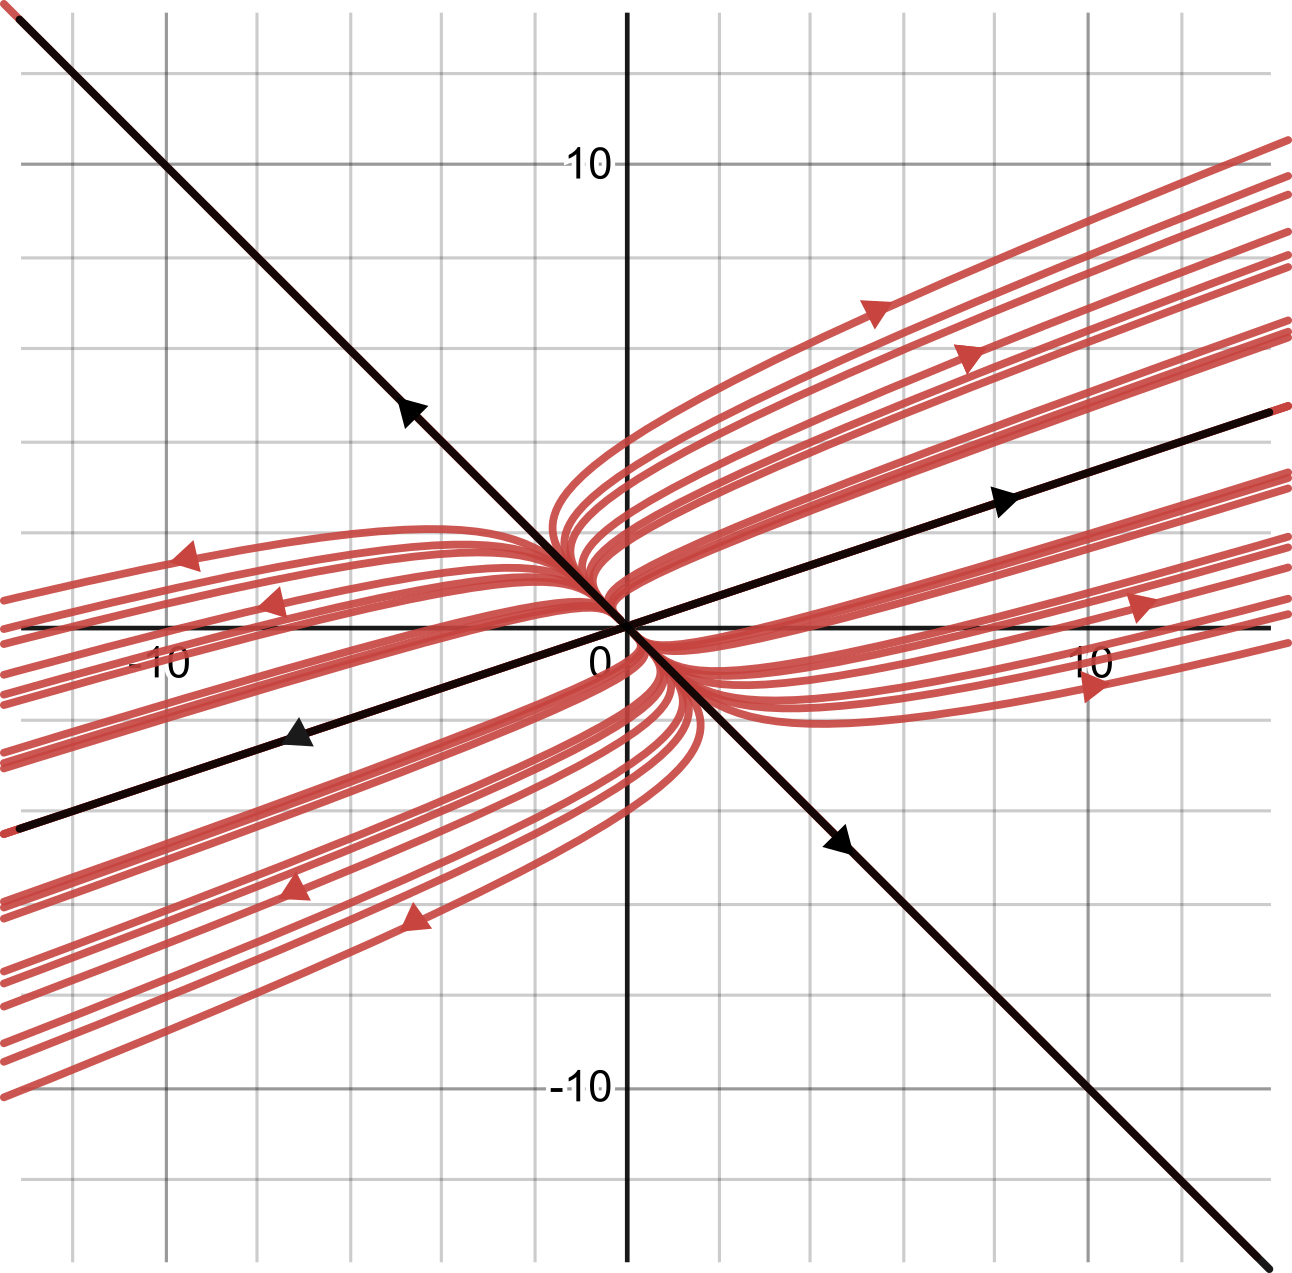
\includegraphics[scale=0.35]{Images/unstable_node.png}
    \caption{Unstable Node}
    \label{fig:unstable_node}
\end{figure}

\subsubsection{Stable Node}
We next look at the case when both eigenvalues are negative. Perhaps unsurprisingly, the picture will be quite similar to the previous with some slight modifications. Continuing our tradition of having a concrete example, we consider
\begin{equation}
    X' = CX
\end{equation}
where $C = A - 5 I$. Our eigenvectors remain $v_1$ and $v_2$ as usual but their corresponding eigenvalues are now $\lambda_1 = -2$ and $\lambda_2 = -6$. Now as we evolve time, everything will approach the origin. Thus we call this situation having a ``stable node at 0". However now $v_2$ approaches the origin faster than $v_1$ so the the integral curves will reflect this by becoming tangent to $v_1$ as $t \to \infty$.
\begin{figure}[h]
    \centering
    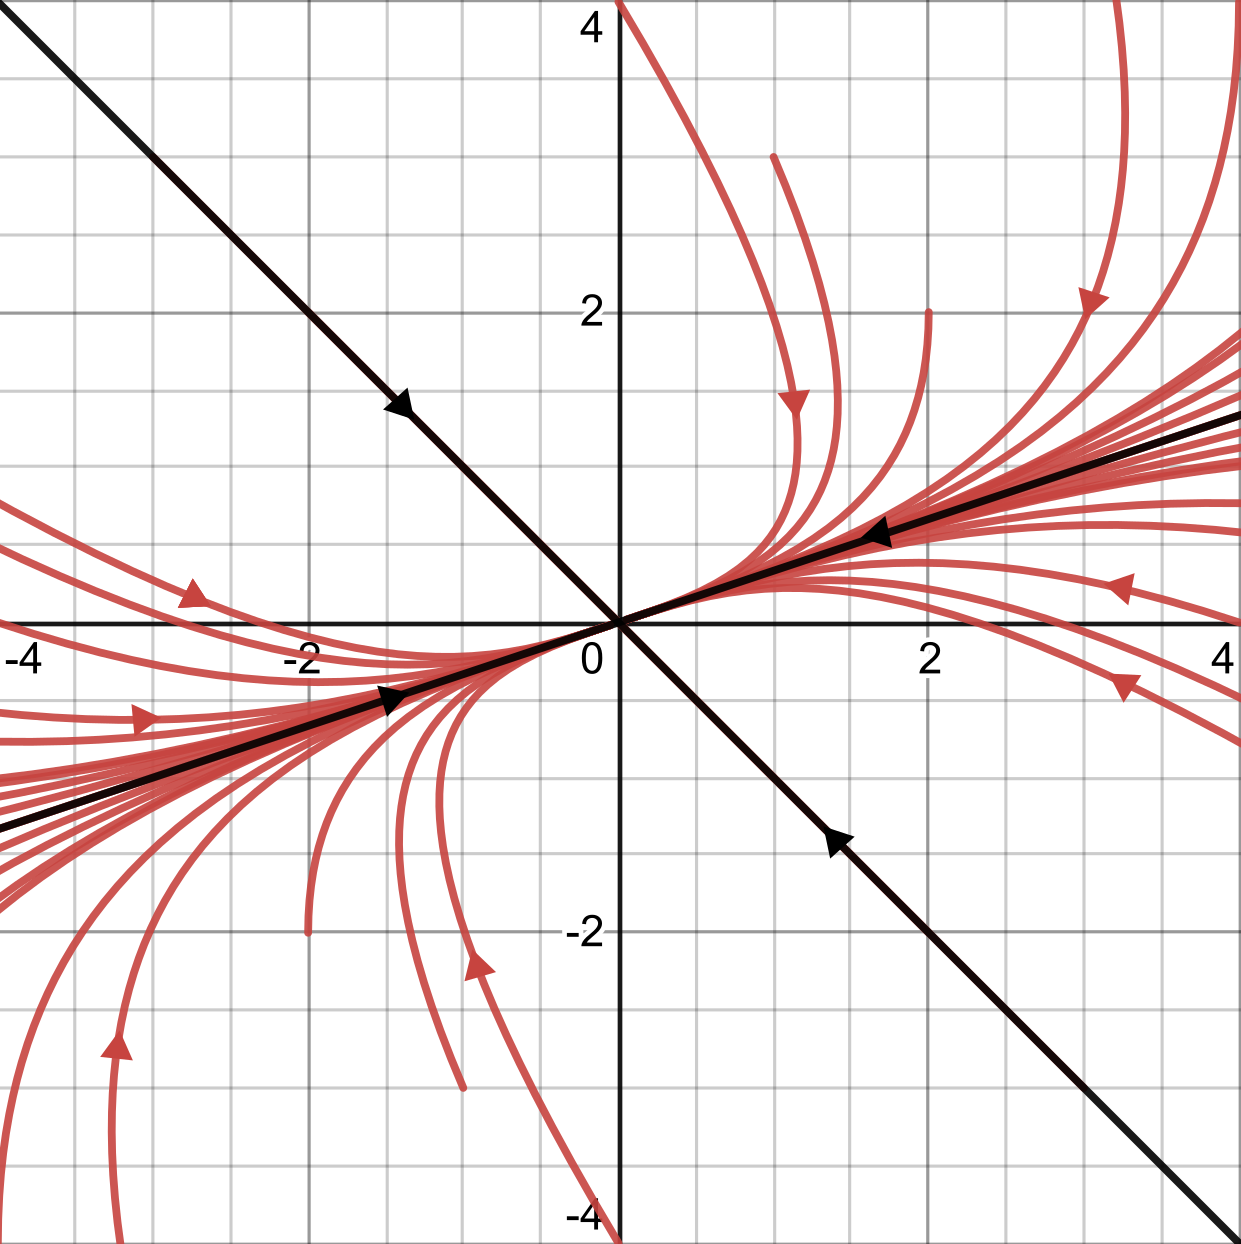
\includegraphics[scale=0.25]{Images/stable_node.png}
    \caption{Stable Node}
    \label{fig:stable_node}
\end{figure}

\subsubsection{Center}
Of course not every real matrix will have eigenvalue. More particularly, it may not have \textit{real} eigenvalues but it will certainly have \textit{complex} eigenvalues. Indeed eigenvalues (for real matrices) come in conjugate pairs. However we can close our eyes, pretend everything is real, and in the end split things into their real and complex complex components to get genuinely real solutions. Let us demonstrate what this means. Suppose we are given
\begin{equation}\label{eq:diff_eqn_center}
    X' = \underbrace{\matrix{0 & -1\\1 & 0}}_{J} X
\end{equation}
In this case, the characteristic equation is $p(\lambda) = \lambda^2 + 1$. The roots of this polynomial are $i$ and $-i$ which are thus our complex eigenvalues. As mentioned, we don't worry about these being complex and proceed as normal. We see that
\begin{align*}
    J - iI = \matrix{-i & -1\\1 & -i}
\end{align*}
and that the vector $v_1 = \matrix{i \\ 1}$ lies in its kernel hence is the corresponding eigenvector for $\lambda_1 = i$. Similarly we conclude $v_2 = \matrix{-i \\ 1}$ is the eigenvector with eigenvalue $\lambda_2 = -i$ (in fact this can be concluded without any calculations. If $A$ is a matrix with real entries and has an eigenvector $v$ with eigenvalue $\lambda$, then $\ol{v}$ is an eigenvector with eigenvalue $\ol{\lambda}$ where $\ol{v}$ is defined in the obvious way: taking the complex conjugate of each entry). Thus our two solutions are
$$ z_1(t) = e^{it} v_1, z_2(t) = e^{-it} v_2  $$
Expanding this using Euler's formula, we get
\begin{align*}
    e^{it} v_1 &= (\cos t + i \sin t) \matrix{i\\1}\\
    &= \matrix{i \cos t - \sin t  \\ \cos t + i \sin t}\\
    &= \matrix{-\sin t \\ \cos t} + i \matrix{\cos t \\ \sin t}
\end{align*}
We claim that
$$X_1(t) = \matrix{-\sin t \\ \cos t}, X_2(t) = \matrix{\cos t \\ \sin t}$$
are (linearly independent) solutions to \autoref{eq:diff_eqn_center} (note we would have gotten the same solutions if we had chose to expand $z_2$ instead).

\begin{figure}[h]
    \centering
    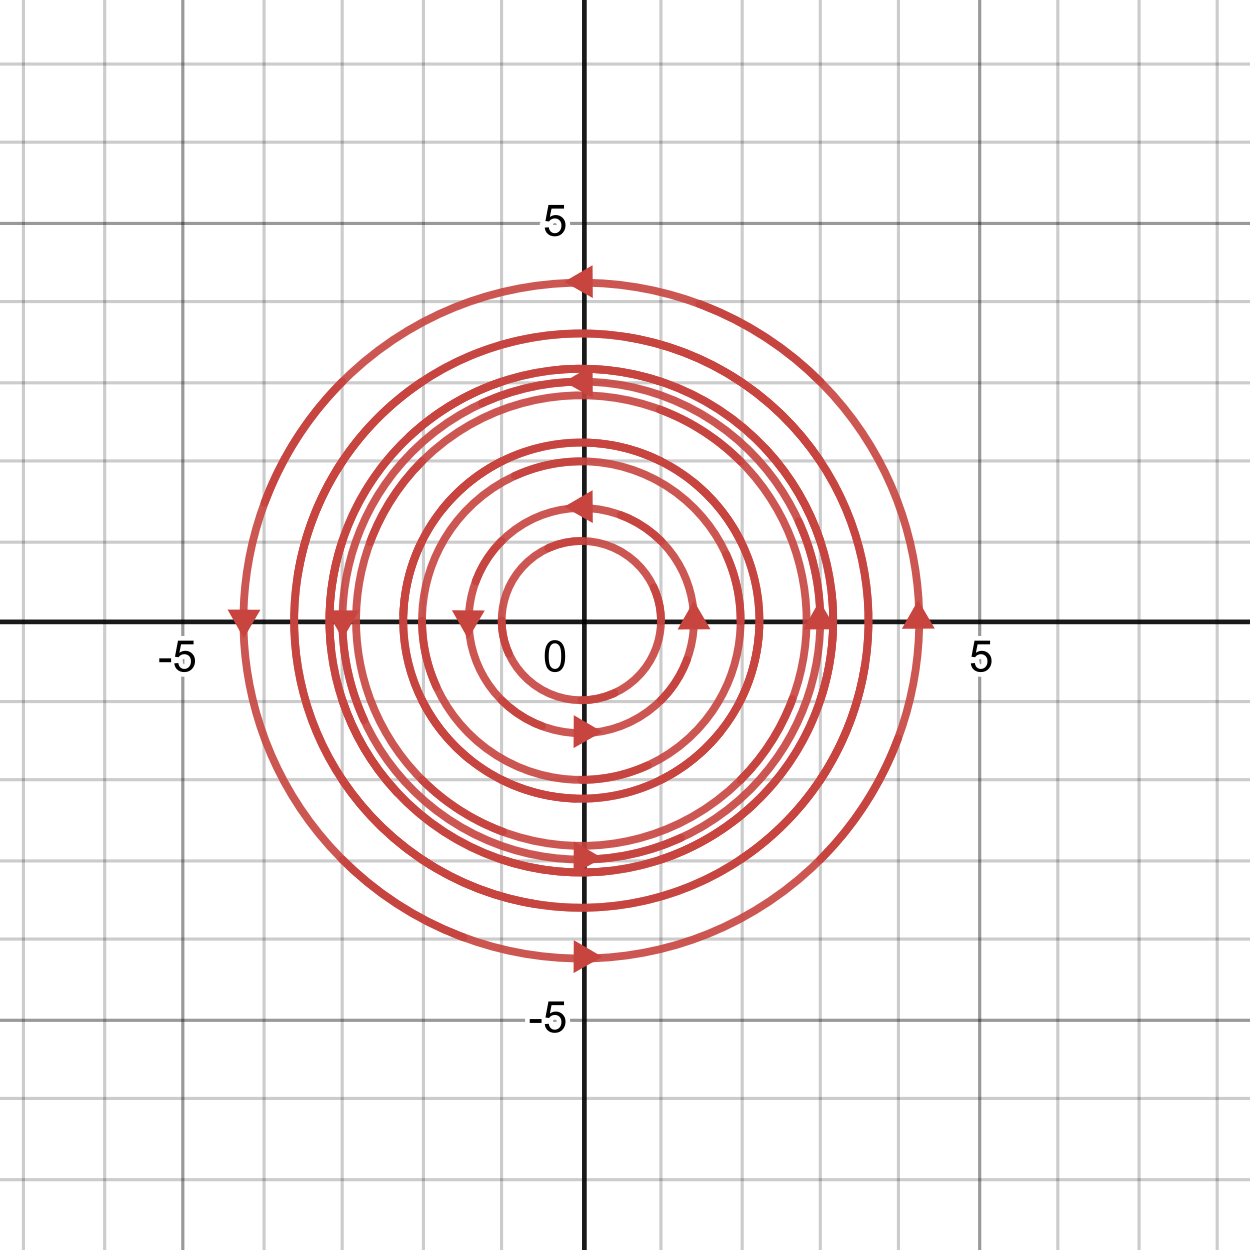
\includegraphics[scale=0.35]{Images/center.png}
    \caption{Center at 0}
    \label{fig:center}
\end{figure}

It is easy to see that the solutions will travel in a circular path: counterclockwise as time moves forward and clockwise as time moves backward. This is known has having a center at 0. This occurs anytime the eigenvalues are purely imaginary numbers.\\

A few claims were made up in the above example. Let us prove them formally.
\begin{lemma}
Suppose $A \in \R^{n \times n}$. Suppose $v$ is an eigenvector with a eigenvalue $\lambda$. Then
\begin{itemize}
    \item $\ol{\lambda}$ is an eigenvalue of $A$ with eigenvector $\ol{v}$
    \item If $\lambda$ is not real, then $v$ is not in $\R^{n}$ (it has complex entries). Moreover, $Re(v)$ and $Im(v)$ are linearly independent.
\end{itemize}
\end{lemma}
\begin{proof}
The first statement is easily verified by noting that $\ol{A} = A$ since $A$ has real entries. Therefore
$$ Av = \lambda v \Leftrightarrow \ol{Av} = \ol{\lambda v} \Leftrightarrow A\ol{v} = \ol{\lambda} \ol{v} $$

In order to verify the second statement suppose $v = u + iw$ where $u, w \in \R^n$. We will prove that $u$ and $w$ are linearly independent via contradiction. So suppose there exists real number $s$ and $t$ and some $v_0 \in \R^n$ such that $u = s v_0$ and $w = t v_0$. Then $v = u + iw = (s + it) v_0$. Since $v_0$ is a multiple of $v$, it must also be an eigenvector of $A$ with eigenvalue $\lambda$. This means that
$$ Av_0 = \lambda v_0 $$
The left side of this equation is always in $\R^n$ however if $\lambda$ is not real then $\lambda v_0$ will not be. Thus we get a contradiction if $\lambda$ is non-real. This shows that $u$ and $w$ are linearly independent so neither can be 0, thus $v$ must have complex entries.
\end{proof}
\begin{lemma}
$Z(t)$ is a complex solution to $X' = AX$ (where $A$ is a real matrix) if and only if $Re(Z(t))$ and $Im(Z(t))$ are also solutions.
\end{lemma}
\begin{proof}
$$ Z_{Re}'(t) + i Z_{Im}'(t) = Z'(t) = A Z(t) = A Z_{Re}(t) + i Z_{Im}(t) $$
\end{proof}